\documentclass[10pt, a4paper, twosize]{article}
%\documentclass[12pt, a4paper, twoside]{book}

\usepackage{helvet}
\usepackage{hyperref}
\usepackage{graphicx}
\usepackage{listings}
\usepackage{textcomp}
\usepackage[
	a4paper,
	outer=2cm,
	inner=4cm,
	top=2cm,
	bottom=2cm
]{geometry}
\usepackage{float}
\usepackage{tabularx}
\usepackage[disable]{todonotes}
\usepackage{color, soul}
\usepackage{amsmath}
\usepackage{algorithmicx}
\usepackage[noend]{algpseudocode}
\usepackage{algorithm}
\usepackage{framed}
\usepackage{subcaption}
\usepackage{titlepic}
\usepackage{fancyhdr}
\usepackage[simplified]{styles/pgf-umlcd}
\usepackage{shorttoc}
\usepackage{url}
\usepackage{paralist}

\definecolor{grey}{rgb}{0.9, 0.9, 0.9}
\definecolor{dkgreen}{rgb}{0,0.6,0}
\definecolor{dkred}{rgb}{0.6,0,0.0}

\lstdefinestyle{DOS}
{
    backgroundcolor=\color{black},
    basicstyle=\scriptsize\color{white}\ttfamily,
    stringstyle=\color{white},
    keywords={}
}

\lstdefinestyle{makefile}
{
    numberblanklines=false,
    language=make,
    tabsize=4,
    keywordstyle=\color{red},
    identifierstyle= %plain identifiers for make
}

\lstset{
  language=Java,                % the language of the code
  basicstyle=\footnotesize\ttfamily,
  numbers=left,                   % where to put the line-numbers
  stepnumber=1,                   % the step between two line-numbers. If it's 1, each line
  numbersep=5pt,                  % how far the line-numbers are from the code
  backgroundcolor=\color{white},      % choose the background color. You must add \usepackage{color}
  showspaces=false,               % show spaces adding particular underscores
  showstringspaces=false,         % underline spaces within strings
  showtabs=false,                 % show tabs within strings adding particular underscores
  frame=single,                   % adds a frame around the code
  rulecolor=\color{black},        % if not set, the frame-color may be changed on line-breaks within not-black text (e.g. comments (green here))
  tabsize=2,                      % sets default tabsize to 2 spaces
  captionpos=b,                   % sets the caption-position to bottom
  breaklines=true,                % sets automatic line breaking
  breakatwhitespace=false,        % sets if automatic breaks should only happen at whitespace
  keywordstyle=\color{blue},          % keyword style
  commentstyle=\color{dkgreen},       % comment style
  stringstyle=\color{dkred},         % string literal style
  columns=fixed,
  extendedchars=true,
  frame=single,
}

%\renewcommand{\chaptername}{Topic}

% New definitions
\algnewcommand\algorithmicswitch{\textbf{switch}}
\algnewcommand\algorithmiccase{\textbf{case}}
\algnewcommand\algorithmicassert{\texttt{assert}}
\algnewcommand\Assert[1]{\State \algorithmicassert(#1)}%
% New "environments"
\algdef{SE}[SWITCH]{Switch}{EndSwitch}[1]{\algorithmicswitch\ #1\ \algorithmicdo}{\algorithmicend\ \algorithmicswitch}%
\algdef{SE}[CASE]{Case}{EndCase}[1]{\algorithmiccase\ #1}{\algorithmicend\ \algorithmiccase}%
\algtext*{EndSwitch}%
\algtext*{EndCase}%

\pagestyle{fancy}
\fancyhf{}
\fancyhead[RO, LE]{\small \rightmark}
\fancyfoot[RO, LE]{\small \thepage}

\begin{document}

%\frontmatter

\begin{titlepage}
\vspace*{5cm}
\begin{center}
\includegraphics[width=.5\textwidth]{images/EdNapUniLogoCMYK}~\\[1cm]

\textsc{\Large Edinburgh Napier University}\\[1.5cm]

\textsc{\LARGE \bfseries SET08122 Algorithms \& Data Structures}\\[0.5cm]

\hrulefill \\[0.4cm]
{\huge \bfseries Lab 1 - Introduction \& Learning Environment \\[0.4cm] }
\hrulefill \\[1.5cm]

\begin{minipage}{0.4\textwidth}
\begin{flushleft} \large
\textbf{Dr Simon Wells} \\
\end{flushleft}
\end{minipage}

\vfill

\end{center}
\end{titlepage}

%\shorttoc{Overview}{0}

%\setcounter{tocdepth}{2}
%\cleardoublepage
%\tableofcontents
%\listoffigures
%\listofalgorithms
%\addtocontents{toc}{~\hfill\textbf{Page}\par}

%\mainmatter

%\input{sections/labs/04_ui}

\section{Aims}
\paragraph{} At the end of the practical portion of this topic you will:

\begin{itemize}
\item Be able to log into the University system
\item Be able to run simple C programs from the command line
\item Be able to run simple programs in another language from the command line
\item Remember how to program simple software
\item Have retrieved some supplementary texts from an online publisher
\end{itemize}


\begin{framed}
{\bf{NOTICE:} This is an introductory lab that is designed to ease ourselves back into programming and make sure that we are comfortable with our learning environment before we start learning new things in earnest. This is partly because the first lab this year is before the first lecture, but also to give a supportive introduction to the module for our direct entrants.}  
\end{framed}


\section{Activities}

\subsection{Writing, Compiling, \& Running C Programs from the Command line}

\paragraph{} The C programming language is our default learning environment for this module. This means that we build on, and consolidate some of the skills that you'll have aquired during the prerequisite Programming Fundamentals module.

\paragraph{} Much of the example code we will be working with is short and simple and doesn't require a complex development environment which can, sometimes, make simple ideas seem much more complicated than necessary. So our default learning environment will be the C programming language. We won't be using an IDE, instead, we'll be working on the command line. The idea is to encourage us to think about every piece of code that we write without too many extra tools that do some of the thinking for us, and to think about the process that turns that code into a running program. We'll actually be going further than this and considering how well our programs run once they are written and compiled. One theme of this algorithms and data structures module is about how the perormance of our programs can depend heavily upon the specific code that we write. It's not good enough to just write code that compiles and runs. Once it runs we want it to run reliably and to compute our results as swiftly as possible

\paragraph{} The toolchain we are going to use is Microsoft’s set of C/C++ compilers, linkers and assemblers. This is mostly because they are pre-installed on university lab machines. However, you could use other C/C++ compilers such as gcc or clang if you are a Linux or Mac OS X user. The code we are using in the first part of the module is standard C with perhaps a smattering of C++ as required.

\subsubsection{Getting an Editor}
\paragraph{} If you are using Microsoft Windows, the text editor we recommend for the module is Notepad++\footnote{\url{http://notepad-plus-plus.org/}}. This editor is free, provides code highlighting, and can be run from a USB key. It is already installed on all of the University machines and can be accessed through Apps Anywhere.

\paragraph{} There are many other text editors exist. Windows comes with Notepad. Linux and Mac OS X come with a variety of tools. Atom, TextWrangler, and SubEthaEdit, are reasonable popular text editors. If you want to get serious about your choice of text editor, which, as adeveloper, is one of your core tools for interacting with a computer, then you might want to consider Vim (or one of it's variants) or Emacs. Both of these tools have complex learning curves but provide huge power to their users. From the point of view of the module, we will not specify a text editor that you must use. It is down to your personal preference. Within lab guidance however we will assume Notepad++.


\paragraph{} In the File menu you can create and save files. For code highlighting to work, you must save the file with the correct extension. For most we will be using C. This means all files should be saved with the .c extension. When using C++ then the .cpp extension will be required. It is also recommended that you save your files somewhere sensible. The H: drive is probably the best place, a USB drive is a good second option, but DropBox, OneDrive, etc. are also options. You are also encouraged to keep your work in a version control repository. We will be using Git as our submission method, e.g. you will submit a git repository, via a clone URL, containing your coursework assignment so you might as well get some extra practise in. Note that one of the activities during this lab is to use Git.

\subsubsection{Using C at the Command Line}
\paragraph{} We will be working from the command line to compile and run our applications. This means you need to open the Visual Studio Developer Command Prompt. To do this, you first need to launch Visual Studio 2017 through Apps Anywhere. Once the Visual Studio main window is open, minimise it (we will not be coding in this window). Then go to the Start Menu, All Programs, Visual Studio 2017, Visual Studio Tools, and choose Developer Command Prompt for VS 2017.
We now need to use some command line instructions to move to the correct folder where you are saving your files. Let us say that you are storing your files on your H drive under a folder called set08122. The commands to use are:

\begin{lstlisting}[style=DOS]
    H:
    cd set08122
\end{lstlisting}

\paragraph{} The first command (H:) changes the drive being accessed to the H drive. The second command (cd set08122) changes the folder to set08122. If you need to go up a directory in the folder structure, you can use the cd .. command. You can find out more about using the command prompt at the Dos Prompt site\footnote{\url{http://dosprompt.info/}} and this is highly encouraged. Whether you work in a Windows, Linux, or Mac environment, you should endeavor to learn as much as you can about the terrain in which you are working.

\paragraph{} As with every introduction to a new programming language we will start with the traditional ``Hello World'' program. Save the following code in a file called hello.c. 

\begin{lstlisting}
#include <stdio.h>
int main(int argc, char **argv) 
{
    printf("Hello world!\n");
}
\end{lstlisting}

\paragraph{} If you copied and pasted that code from the labsheet then you may encounter problems. At the very least you might experience badly formatted code, at worst you will find that you've copied non-printing characters which could break your program or introduce more subtle bugs. It is much better to your code in yourself. At minimum this means that you are getting deliberate practise of the language, yes, it is slower than copying and pasting, but typing makes you spend time on every character of every line of the program which is an important part of the learning process.

\paragraph{} We are now ready to compile our application. To do this we are using Microsoft’s C/C++ compiler - cl. We will visit some of the different commands we can give cl through the module. For the moment we will perform the simplest task - having cl build an executable from a single .c file. The command to do this is as follows:

\begin{lstlisting}[style=DOS]
       cl hello.c
\end{lstlisting}

\paragraph{} You should now see output similar to the this:

\begin{lstlisting}[style=DOS]
Microsoft (R) C/C++ Optimizing Compiler Version 18.00.30501 for x86 
Copyright (C) Microsoft Corporation. All rights reserved.

hello.c
Microsoft (R) Incremental Linker Version 12.00.30501.0
Copyright (C) Microsoft Corporation. All rights reserved.

/out:hello.exe 
hello.obj
\end{lstlisting}

\paragraph{} Read the output that you got. If there is an error in your source code then the compiler will very likely have caught it and tried to tell you about it, for example, perhaps mentioning a ``syntax error''. Read error messages carefully and try to work out where the problem lies. This is an important skill to develop as, during your career, you will make a lot of coding errors over the years.

\paragraph{} Once you have a compiled file, run it by typing \emph{hello} at the command prompt:


\begin{lstlisting}[style=DOS]
    hello
    Hello world!
\end{lstlisting}

\paragraph{} Well done. If you hadn't already done so, you just wrote your first C program. There is obviously a lot more to know so you should do some practice C programming. Later in this lab there are links to some programming practice sites that provide programming challenges so that you don't have to work out programs to write for yourself. This will help you practise and to learn new syntax. We'll obviously get lots of opportunities to then apply this over the coming weeks.

\subsection{Additional Languages}
\paragraph{} Both Python and Java are available on University lab machines amongst other choices. As we progress through the module you are encouraged to explore how the topics we cover in C translate through to at least one other language of your choice. It is not a bad idea to select the language that you are most comfortable with.

\subsubsection{Python}
\paragraph{} Python is available in the Napier Labs. Select the following icon

\includegraphics{images/software_icon}

\paragraph{} In the window that opens, scroll through until you find Python. It should look something similar to this:

\includegraphics[width=.8\textwidth]{images/sofware_window}

\paragraph{} Double click the Python icon and a Python shell should open. This shell is a Read-Evaluate-Print-Loop, known as a REPL (usually pronounced \emph{re-pul}). You can type in Python code and it will be processed and the result printed to the screen. The shell should look like this:

\includegraphics[width=.8\textwidth]{images/python_repl}

\paragraph{} If you've not used Python before but want to give it a go then I'd suggest quickly skipping to the background reading section, downloading ``Data Structures and Algorithms with Python'' then returning here and working through the first chapter which gives a quick introduction to Python. 

\paragraph{} Alternatively, you could learn some Python by exploring some of the excellent online `learn Python' tutorials that are available. Some of them are interactive, so you can type directly into the web-site and get results. Others just give you exercises to do yourself and you can do those exercises in Python on our Levinux platform. Here are a few, in order of usefulness according to me, but many more are just a Google search away:

\begin{enumerate}
\item Learn Python the hard way: \url{http://learnpythonthehardway.org/book/}
\item The Python Practice Book: \url{http://anandology.com/python-practice-book/index.html}
\item A Byte of Python: \url{http://www.swaroopch.com/notes/python/}
\item Code Combat: \url{https://codecombat.com/}
\item Python for you and me: \url{http://pymbook.readthedocs.org/en/latest/}
\item The Hitchhiker's Guide to Python:\\ \url{http://docs.python-guide.org/en/latest/#the-hitchhiker-s-guide-to-python}
\item Hands-On Python Tutorial: \url{http://anh.cs.luc.edu/python/hands-on/3.1/handsonHtml/index.html}
\item The Python Challenge: \url{http://www.pythonchallenge.com/} - Some quite touch challenges that you can solve using Python (NB. Assumes you already know what you are doing)
\item Python Tutor: \url{http://www.pythontutor.com/} - Helps visualise the execution of Python code. Again, assumes that you have some prior knowledge of Python syntax.
\end{enumerate}

\paragraph{} The links towards the top of the list are aimed at those completely new to the Python language whereas those further down the list will help those who have some Python knowledge already.

\subsubsection{Java}

\paragraph{} The Java JDK is already installed on lab machines. Open a new command line by navigating to the start menu and typing in cmd.exe then pressing return.


\includegraphics[width=.8\textwidth]{images/start_cmd}

\paragraph{} Your new terminal should look like this:

\includegraphics[width=.8\textwidth]{images/cmd}

\paragraph{} If you type javac and press return and get the following output:

\begin{lstlisting}[style=DOS]
    C:\>javac
    'javac' is not recognized as an internal or external command,
    operable program or batch file.
    C:\>
\end{lstlisting}

\paragraph{} then you need to set your path. Type the following into the command line then press return:

\begin{lstlisting}[style=DOS]
    C:\> set "path=%path%;c:\program files\Java\jdk1.8.0_121\bin"
\end{lstlisting}


\paragraph{} This will have set the path to the JDK for this session. Do some google research to discover how to set this permanently using an environment variable, but for now this will suffice. However you may need to reset your path each time you open a new command line.

\paragraph{} You can now run a simple Java program by typing some Java source code into a file, saving it then compiling and running it from the command line, e.g.

\begin{lstlisting}
public class HelloWorld {

	public static void main(String[] args) {
		System.out.println("Hello Algorithms & Data Structures");
	}
}
\end{lstlisting}

\paragraph{} You should now be able to type something similar to the following (assuming you named your file ``HelloWorld.java'':

\begin{lstlisting}[style=DOS]
    C:\> javac HelloWorld.java
    C:\> java HelloWorld
\end{lstlisting}

\paragraph{} This should of course be familiar to all of us, but a refresher never hurt anyone.

\subsection{Practice Programming}

\paragraph{} You can use any language that you like so use the opportunity to either practise a language you alread know or else to learn a new language. Remember, the more code that you write then the better you will be and the more your skills will improve. The best coders whom I have had the opportunity to work with were all good programmers purely because they put a lot of time and effort into getting better at what they do. 

\paragraph{} The task is to work through as many problems from [Project Euler](https://projecteuler.net/) as you like. Make sure to create a Git repository and add the code that you write for each problem to your repo. then push it to your remote account (Bitbucket or Github).

\paragraph{} I often use established problem lists as a way to learn a new language or to practise one I already know. There are many other similar sites that provide problem sets so if you can't think of a program to write then these places are a good starting point:

\begin{description}
\item[Project Euler]\url{https://projecteuler.net/}
\item[Stack Exchange Code Golf]\url{http://codegolf.stackexchange.com/}
\item[Code kata]\url{http://codekata.com/}
\item[Reddit Daily Programmer]\url{https://www.reddit.com/r/dailyprogrammer}
\item[Programming Praxis]\url{http://programmingpraxis.com/}
\item[Rosetta Code]\url{http://rosettacode.org/wiki/Main_Page}
\item[International Collegiate Programming Contest Problems Index]\url{http://acm. hit.edu.cn/judge/ProblemIndex.php}
\item[Algorithmist]\url{http://www.algorithmist.com/index.php/Main_Page}
\end{description}


\subsection{Background Reading}

\paragraph{} Use your browser to visit \url{http://link.springer.com}. If you are on the university network you shouldn't have to log in, but otherwise your university credentials will work with the Shibboleth log in option on the site. Use the search option with the following query: ``Algorithms and Data Structures'', you might want to narrow the result by selecting the ``Books'' option in the menu on the lefthand side.

\paragraph{} You can, and should, download PDF copies of the following books which will supplement your reading throughout the module. However there are many books on this topic and you are encouraged to try out lots of texts until you find something that you can read easily. It is also a good idea to try to read the same topic repeatedly in multiple texts as each text will have a different emphaisis, assume different underlying knowledge, and overlap in different ways, so you are more likely to build a comprehensive and deep understanding by using multiple sources. Note taht there are also many blogs and websites that deal with data structures which can also supplement your learning.

\begin{itemize}

\item Data Structures and Algorithms: \emph{A First Course}\\
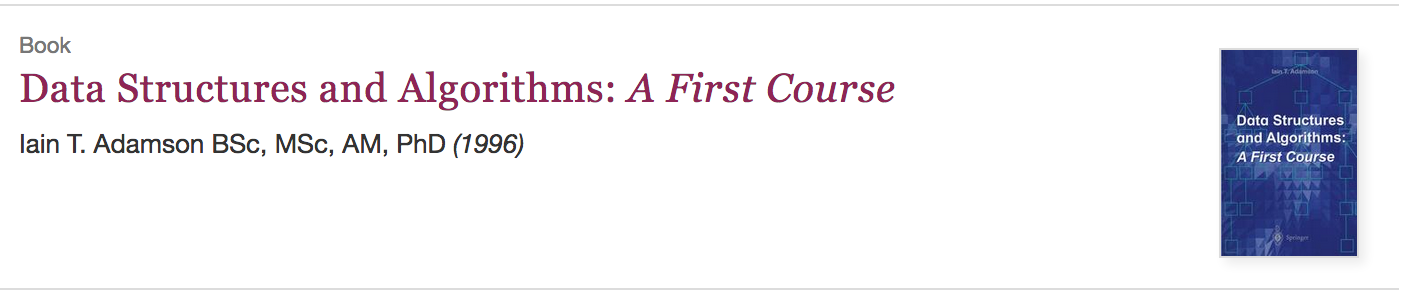
\includegraphics[width=.8\textwidth]{images/adamson}

\item Algorithms and Data structures: The Basic Toolbox\\
\includegraphics[width=.8\textwidth]{images/mehlhorn}

\item An Introduction to Data Structures and Algorithms\\

\includegraphics[width=.8\textwidth]{images/storer}

\item Data Structures and Algorithms with Python\\
\includegraphics[width=.8\textwidth]{images/lee}

\item A Concise and Practical Introduction to Programming Algorithms in Java\\
\includegraphics[width=.8\textwidth]{images/nielsen}

\end{itemize}

\paragraph{} Pointers to other texts, chapters, and papers will be suggested throughout the module, but these should be enough to get started and provide a solid underpinning for your learning.

\subsection{Use Git}

\begin{framed}
\textbf{IMPORTANT} Git is used for coursework submission so you should get familiar with it as soon as possible if you are at all unsure. Use the demonstrators experience and knowledge to help you if you're stuck.
\end{framed}

\paragraph{} Git is a source control system that enables you to keep track of your source code, its history and any changes you make. Git can be used to track any file but is most efficient and best suited when used only with textual files. Because Git is a \emph{distributed} source control system it works very well to enable groups of people to work on the same source code as well as supporting experimenting with your code, trying out lots of different ideas in separate \emph{branches} (which are a bit like a copy of your code but with tools to help manage that copy and support re-integrating it with your main source tree if you want to), and being able to roll back to an earlier version if you decide you have take a wrong turn.

\paragraph{} There are a number of options for setting up Git on the lab machines, but a good place to start is with the ``Using Git for Napier Students'' document\footnote{\url{https://www.dropbox.com/s/2kz34u0zb4qajvd/getting.started.pdf?dl=1}}. For additional information about using Git, a good place to start is by dipping into the Git SCM book\footnote{\url{http://git-scm.com/book/en/v2/Getting-Started-About-Version-Control}}.


\paragraph{} There are also numerous interactive tutorials and resources to help you get started with Git:
\begin{enumerate}
\item Github's Learn Git 15 minute tutorial: \url{https://try.github.io/levels/1/challenges/1}
\item Learn Git Branching \url{http://pcottle.github.io/learnGitBranching/}
\item Git Immersion \url{http://gitimmersion.com/lab_01.html}
\end{enumerate}

\paragraph{} It is worth working through at least one of these tutorials to get some hands-on training. Using Git is a professional skill that it is worth developing if you are going to be writing code.

\paragraph{} You should also create either a Github account\footnote{\url{https://github.com/}} or a Bitbucket account\footnote{\url{https://bitbucket.org}} (or both if you like) then create a repository within your new account called `set09117'. You will push all of your code throughout the module into this repository and at hand in time I will pull a copy for marking. The advantage of this appraoch is that at any point, if you need help with your code, then we have a copy that I can see remotely. However this only works if you keep adding your code to your repository. That means whenever you make changes you need to (1) add them, (2) commit them with an explanatory message,  and (3) push the changes from your local repository to the shared one on Github or Bitbucket.



%\backmatter

\bibliographystyle{plain}

\bibliography{workbook}

\end{document}

%\begin{framed}
%HELLO
%\end{framed}



